\documentclass[9pt]{beamer}
\usepackage[ngerman]{babel}
\usepackage{bibgerm}
\usepackage{bibentry}
\usepackage[autostyle]{csquotes}
\usepackage{siunitx}

\usetheme{TUDOplain}
\setbeamertemplate{navigation symbols}{}
\setbeamercovered{invisible}
\makeatletter
\renewcommand\@makefnmark{%
	[\@thefnmark]}
\renewcommand\@makefntext[1]{%
	\noindent\tiny [\@thefnmark] #1}
\makeatother
\setbeamertemplate{footline}{\small \vspace{-1ex} \vbox{ \insertframenumber /\inserttotalframenumber}}

\sisetup{
	locale = DE ,
	per-mode = fraction,
	binary-units = true 
}
\DeclareSIUnit\pixel{px}

\author[Merlin Scholz]{Merlin Scholz\\\href{mailto:merlin.scholz@tu-dortmund.de}{merlin.scholz@tu-dortmund.de}}
\title[Analyse der Marsoberfläche durch Unsupervised Learning]{Kategorisieren der Marsoberfläche mithilfe von Unsupervised Learning durch Backpropagation}
\date[20.11.2019]{20. November 2019}
\institute[TU Dortmund]{Mustererkennung,\\Informatik XII, Technische Universität Dortmund}

\begin{document}

\begin{frame}
\titlepage

\bibliographystyle{gerabbrv3}
\nobibliography{presentation.bib}
\end{frame}

\begin{frame}{Inhalt}
	\tableofcontents
\end{frame}

\section{Motivation}

\begin{frame}{Motivation: Neuronale Netze zur Bildsegmentierung}
\begin{columns}
	\begin{column}{.5\textwidth}
		\begin{itemize}
			\item Neuronale Netzwerke werden oft zur Bildsegmentierung genutzt
			\item Voraussetzung: Manuell erstellte Ground Truth um das Netzwerk zu trainieren
			\end{itemize}
	\end{column}
	\begin{column}{.5\textwidth}
		\begin{figure}[H]
			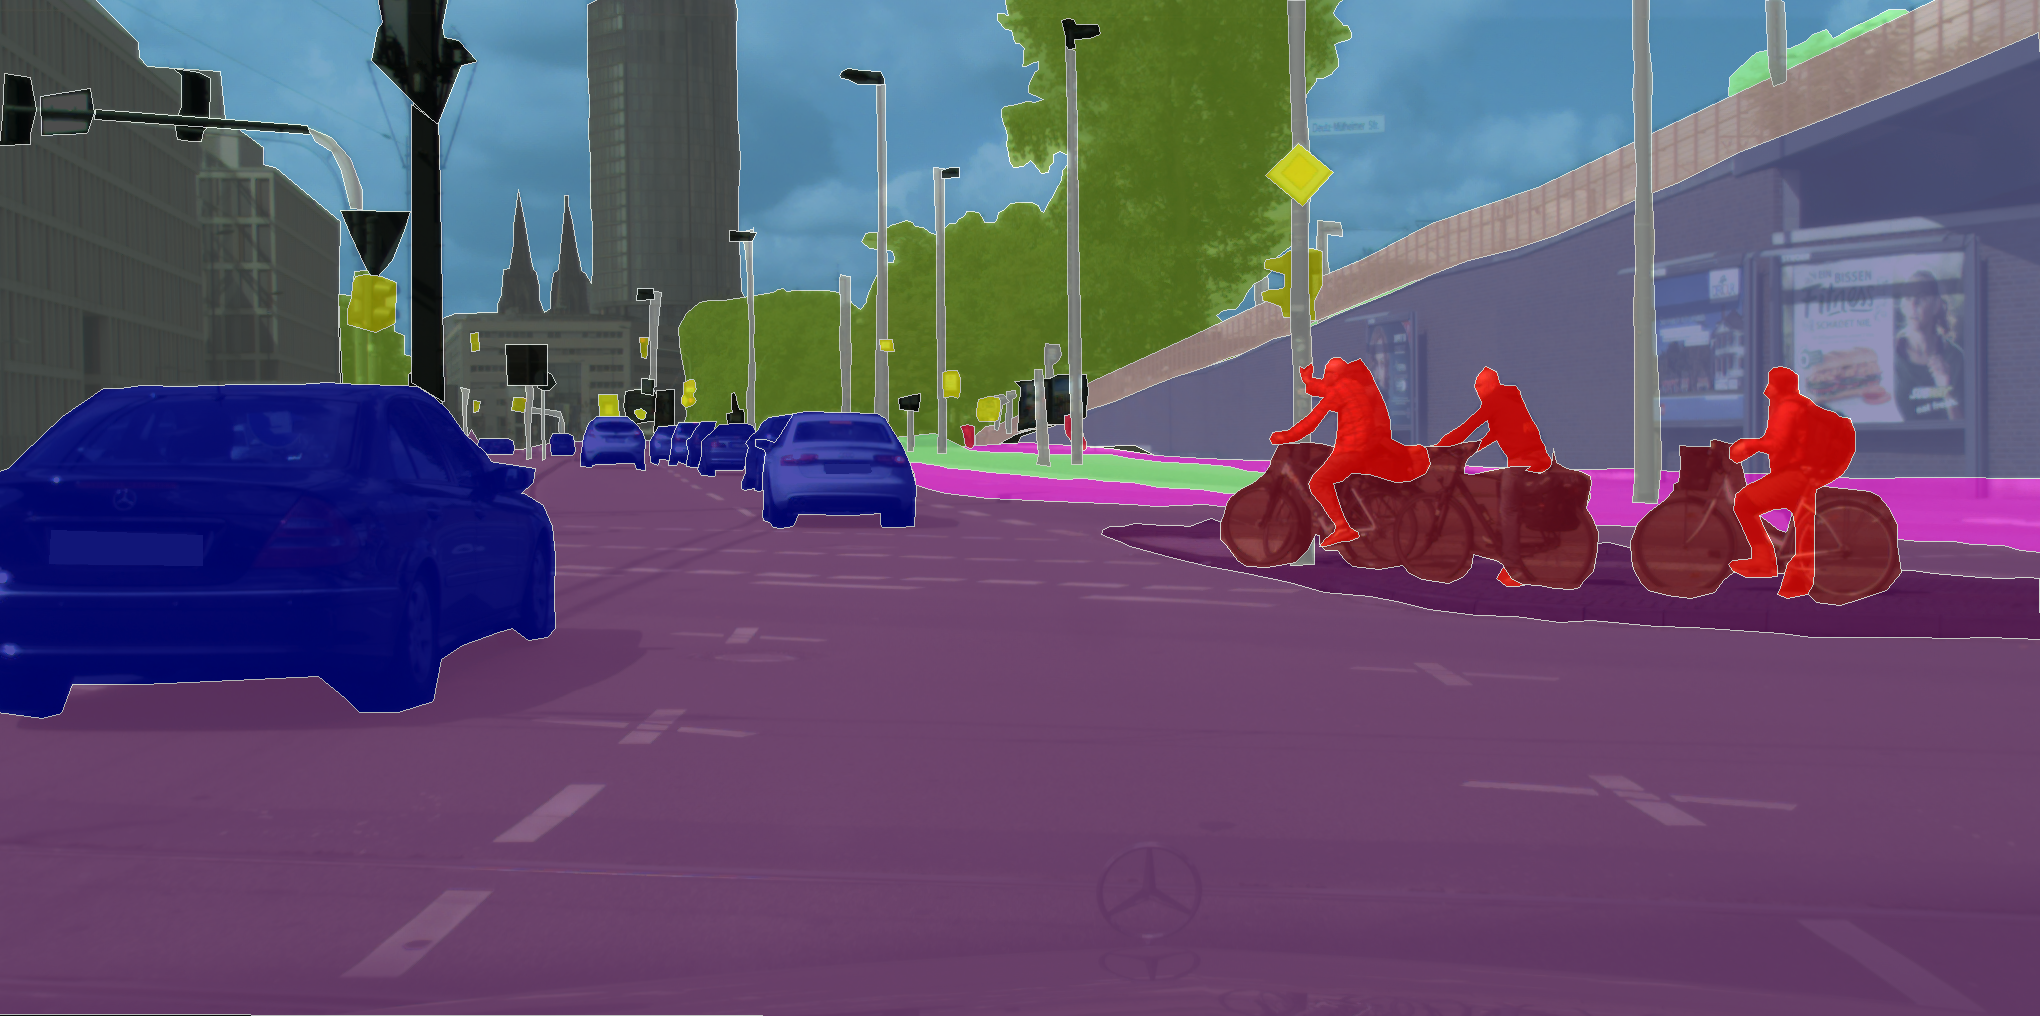
\includegraphics[width=\textwidth,keepaspectratio]{koeln00.png}
			\caption{Beispiel: CityScapes Dataset\footnotemark[1] }
		\end{figure}
	\end{column}
\end{columns}
\footnotetext[1]{\bibentry{Cordts_2016_CVPR}}
\end{frame}

\begin{frame}{Motivation: (Fehlende) Ground Truths}
Ground Truth nicht immer vorhanden: Beispiel Marsoberfläche
\begin{itemize}
	\item Zu großer Datensatz
	\item Notwendigkeit von Experten
	\item[$\Rightarrow$] Manuelle Erstellung nicht kostengünstig oder zeiteffizient möglich
\end{itemize}
\medskip
Lösungsansatz:
\begin{itemize}
	\item Anfangs zufällige Klassifizierung durch Segmentierungsalgorithmus weiter optimieren
\end{itemize}
\end{frame}

\section{Verwandte Arbeiten}

\begin{frame}{Verwandte Arbeiten: Segmentierung nach Kanezaki\footnotemark[1] (1)}
\begin{itemize}
	\item Unüberwachtes Lernen der Segmentierung
	\item Anfangs zufällige Ergebnisse werden mit Clusteringalgorithmus (hier SLIC\footnotemark[2]) vereint
	\item Zielfunktion: Softmax-Loss zwischen Ergebnis des NN und des optimierten Ergebnisses
	\item NN wird auf diese Zielfunktion hin optimiert (Backpropagation)
\end{itemize}
\footnotetext[1]{\bibentry{kanezaki2018_unsupervised_segmentation}}
\footnotetext[2]{\bibentry{slic}}
\end{frame}

\begin{frame}{Verwandte Arbeiten: Segmentierung nach Kanezaki\footnotemark[1] (2)}
\begin{figure}
	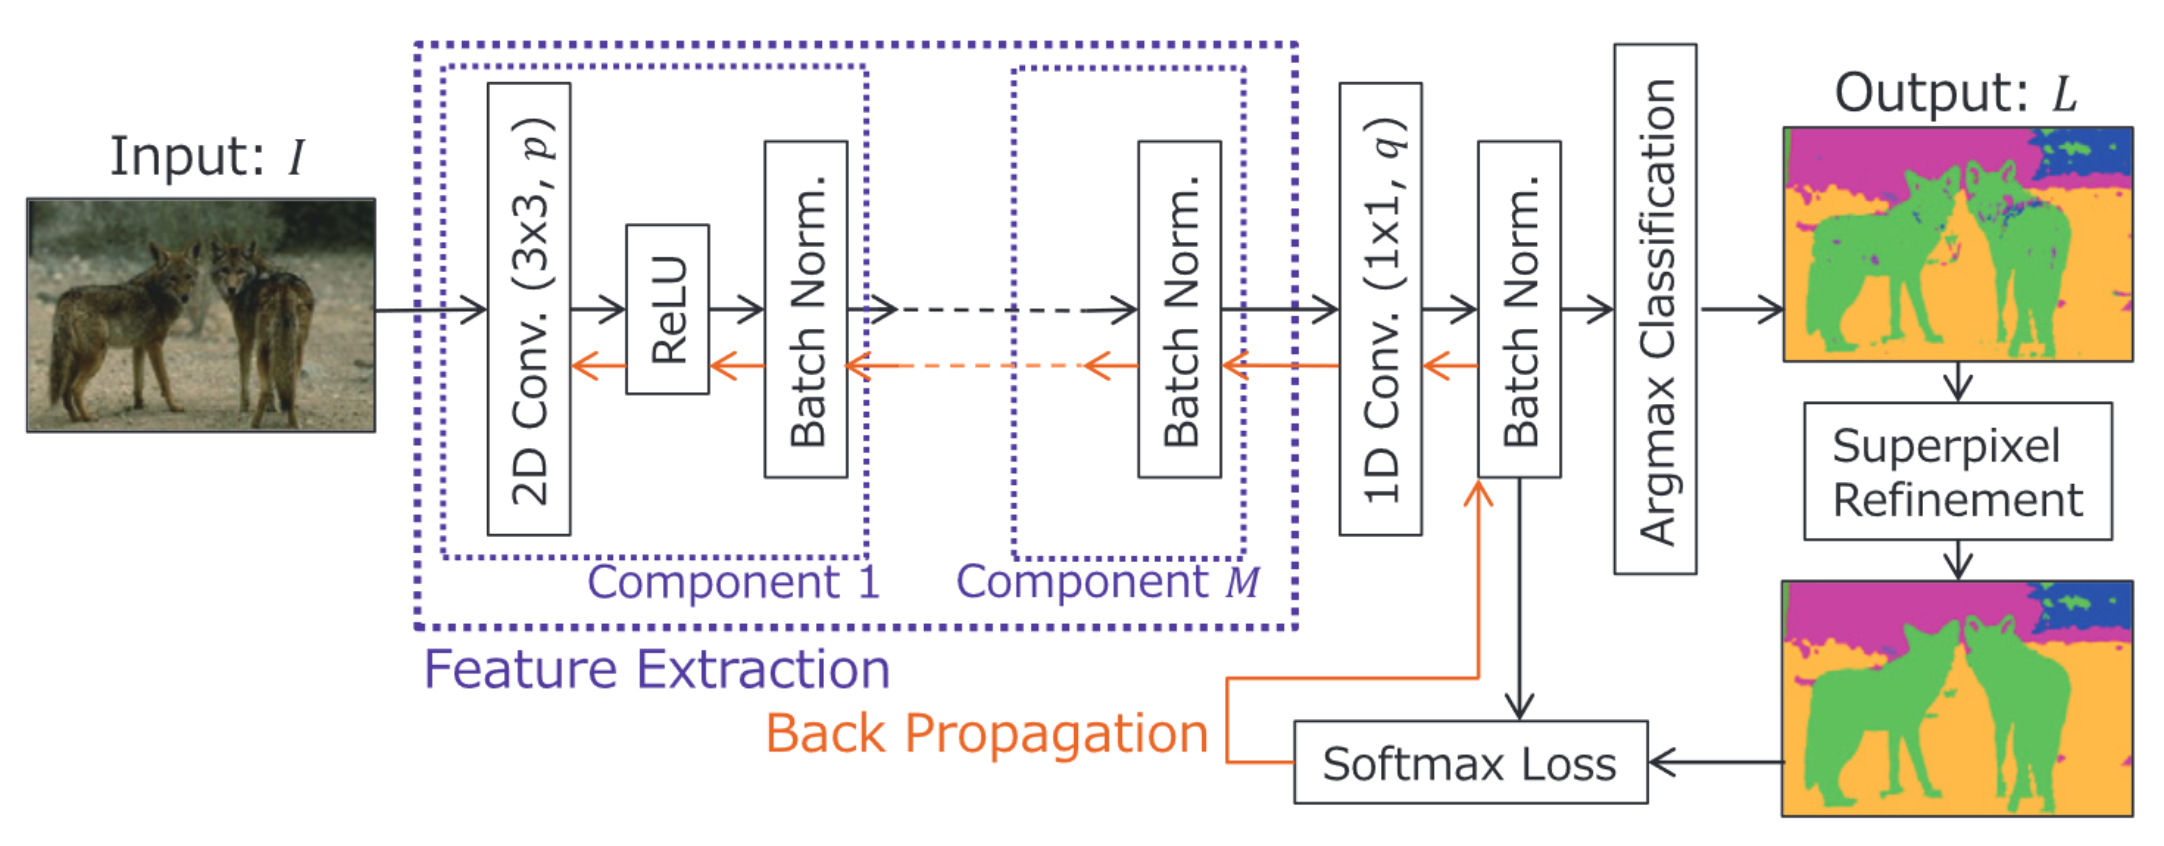
\includegraphics[width=\textwidth,keepaspectratio]{kanezaki.png}
	\caption{Vorgehensweise nach Kanezaki}
\end{figure}
\footnotetext[1]{\bibentry{kanezaki2018_unsupervised_segmentation}}
\end{frame}

\begin{frame}{Verwandte Arbeiten: Segmentierung nach Kanezaki\footnotemark[1] (3)}
\begin{figure}
	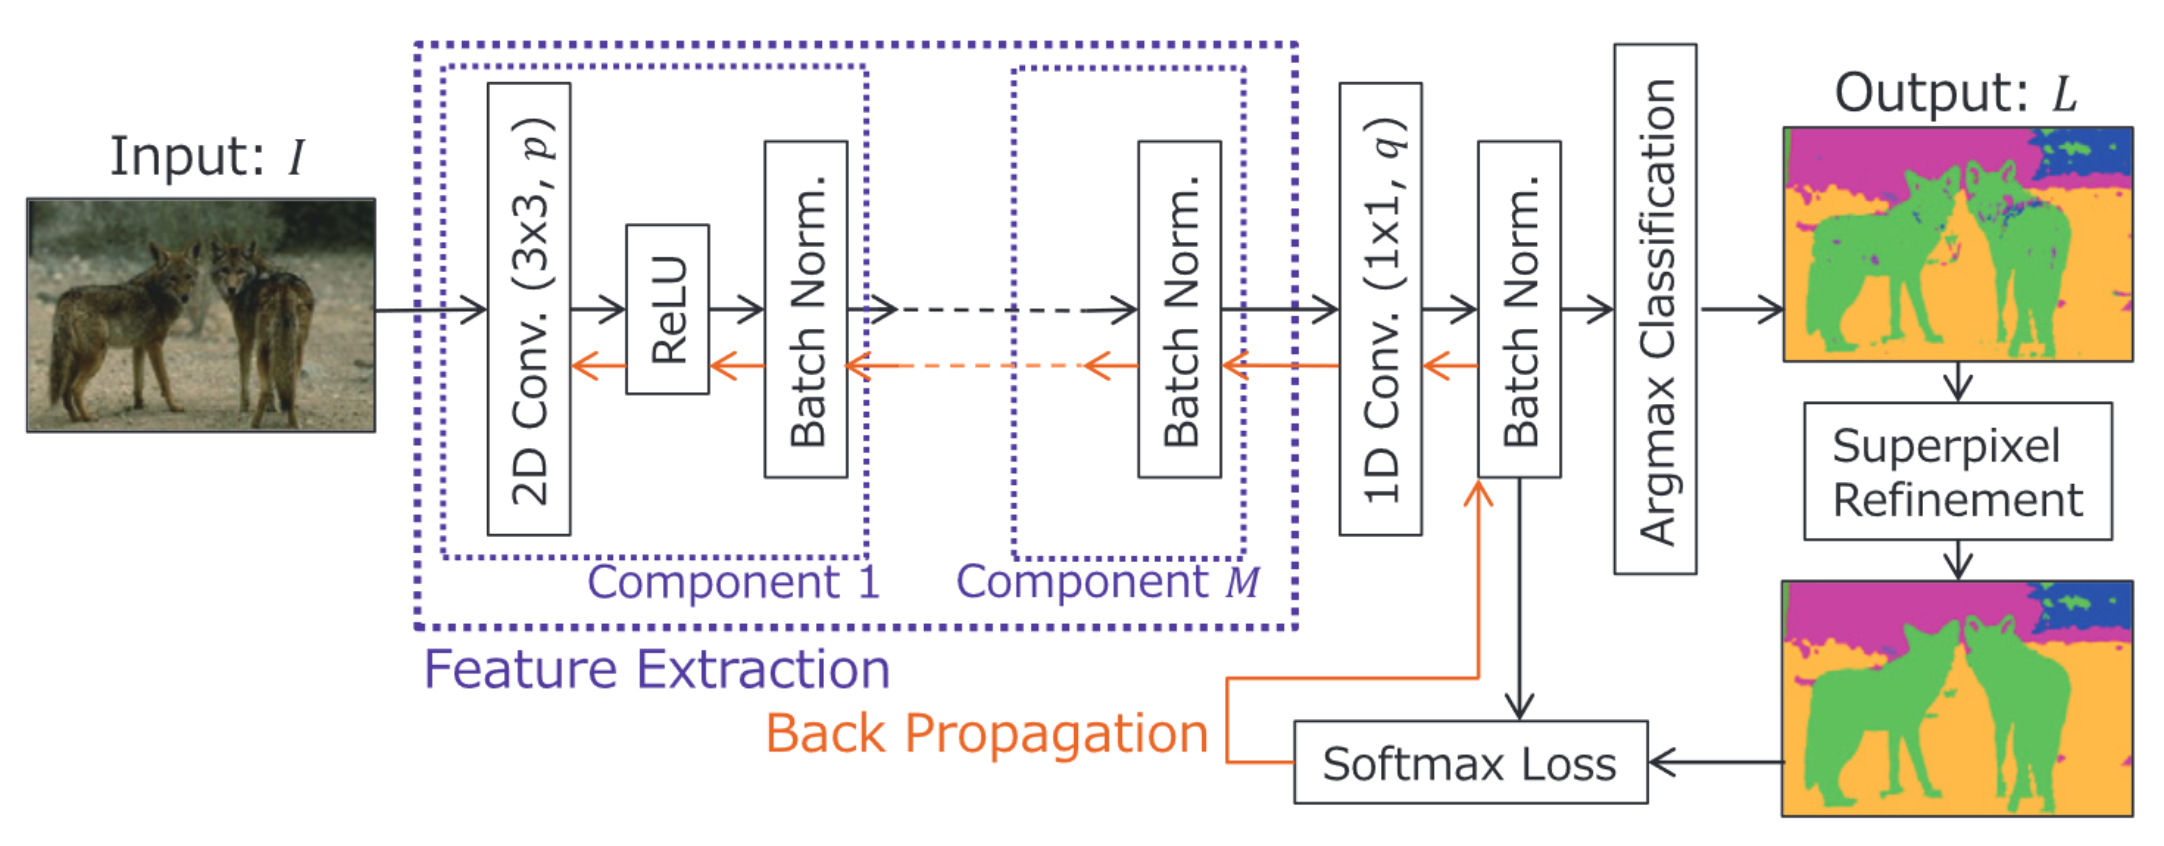
\includegraphics[width=\textwidth,keepaspectratio]{kanezaki.png}
	\caption{Vergleich zwischen klassichem SLIC-Algorithmus und Ansatz von Kanezaki}
\end{figure}
\footnotetext[1]{\bibentry{kanezaki2018_unsupervised_segmentation}}
\end{frame}

\begin{frame}{Verwandte Arbeiten: \textit{Deep Embedded Clustering[...]}}
	\begin{columns}
		\begin{column}{.5\textwidth}
			\begin{itemize}
				\item TODO
			\end{itemize}
		\end{column}
		\begin{column}{.5\textwidth}
			\begin{figure}
				
			\end{figure}
		\end{column}
	\end{columns}
\end{frame}

\begin{frame}{\textit{Detection of craters [...] using shape and texture features} nach Bandeira\footnotemark[1]}
\begin{columns}
	\begin{column}{.5\textwidth}
		\begin{enumerate}
		\item Vorsortierung basierend auf Urbach \& Stepinskis Algorithmus\footnotemark[2] zur Kratererkennung
		\begin{itemize}
			\item Effiziente Methode zur Krater-Erkennung
			\item $\SI{70}{\percent}$ Erkennungsrate
			\item Funktionsweise über Schatten und Highlights
		\end{itemize}
		\item Überlagerung von 9 Bitmasken (in versch. Positionen) und Prüfung auf Übereinstimmungen
		\item Anwendung eines angepassten AdaBoost Algorithmus
		\item Post-Processing: Eliminierung von ungewöhnlich geformten Kratern
		\end{enumerate}
	\end{column}
	\begin{column}{.5\textwidth}
		\begin{figure}[H]
			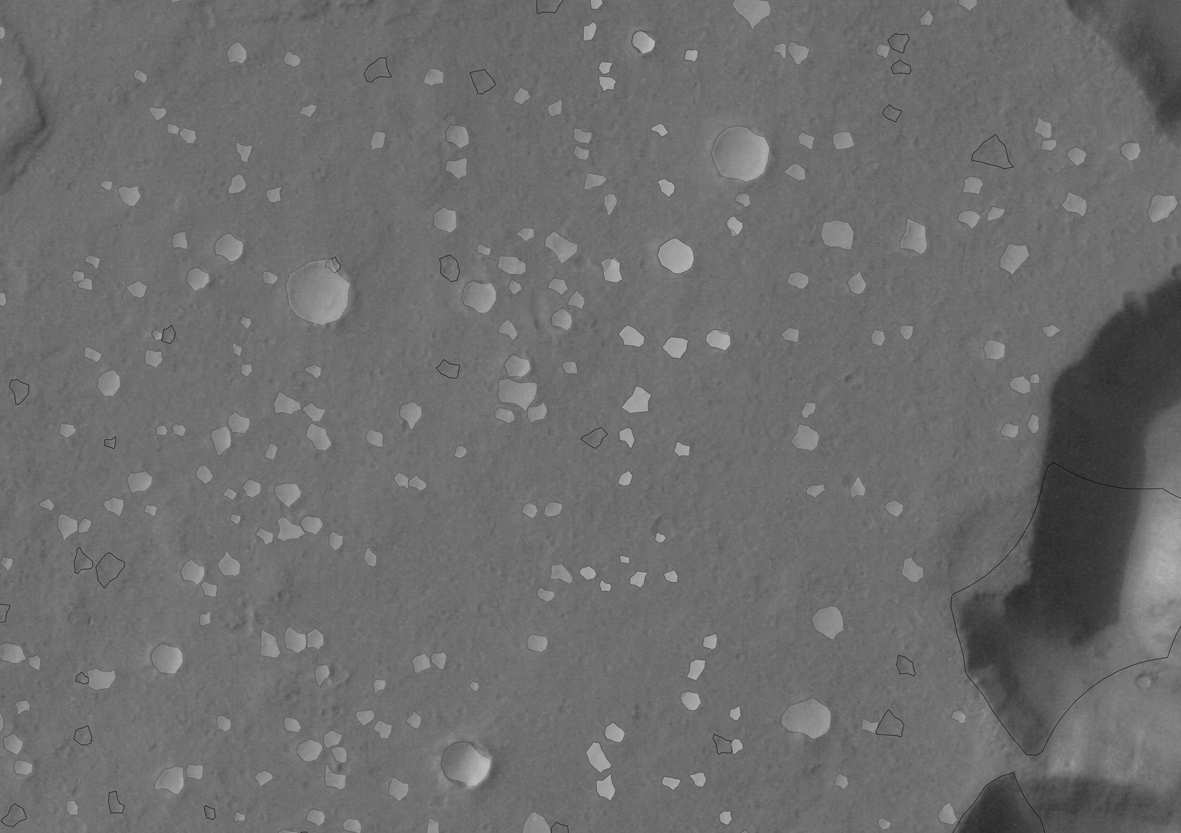
\includegraphics[width=\textwidth, keepaspectratio]{bandeira_detected.png}
			\caption{Erkannte Krater nach Bandeira}
		\end{figure}
	\end{column}
\end{columns}
\bigskip
\begin{center}Hierauf basierend: Der Krater-Datensatz der University of Massachusetts\footnotemark[3]\\
	(vergleichbar mit unserem Ziel)
\end{center}

\footnotetext[1]{\bibentry{Bandeira2012}}
\footnotetext[2]{\bibentry{urbach2009automatic}}
\footnotetext[3]{\bibentry{umass_craters}}
\end{frame}

\begin{frame}{Verwandte Arbeiten: \textit{Crater Detection via CNNs}\footnotemark[1]}
\begin{itemize}
	\item Erforscht Neuronale Netze statt manuell erstellten Filtern
	\item \enquote{Klassischer} Ansatz über neuronale Netze
	\item Lernt auf Bandeira-Datensatz der UMass
	\item Nutzt F1-Score und Cross Validation zur Evaluierung
	\item Gute Ergebnisse, F1-Score zwischen $\SI{88}{\percent}$ und $\SI{91}{\percent}$ (vgl. Bandeira $\SI{79}{\percent}-\SI{86}{\percent}$)
\end{itemize}
\footnotetext[1]{\bibentry{2016arXiv160100978C}}
\end{frame}

\section{Problemstellung}

\begin{frame}{Problemstellung: Datensatz}
\begin{columns}
	\begin{column}{.7\textwidth}
		\begin{itemize}
			\item Eingabedaten sind Bilder der Kameras des Mars Reconnaissance Orbiters
			\begin{itemize}
				\item \alert{Context-Camera (CTX-Kamera) für allgemeine Terrain-Übersicht $\SI{6}{\meter\per\pixel}$}
				\item \textit{High Resolution Imaging Experiment} (HiRISE) für genauere Detailaufnahmen
			\end{itemize}
			\item CTX-Streifen jeweils $\sim\SI{150}{\mebi\byte}$ groß, Auflösung bis zu $\SI{10000}{px}*\SI{30000}{px}$
			\item Insgesamt etwa $\SI{13}{\tebi\byte}$ an Daten
			\begin{itemize}
				\item[$\Rightarrow$] Manuelle Segmentierung nicht möglich
				\item[$\Rightarrow$] Algorithmus sollte effizient sein
				\item[$\Rightarrow$] Algorithmus sollte minimal menschliche Überwachung benötigen
			\end{itemize}
		\end{itemize}
	\end{column}
	\begin{column}{.3\textwidth}
		\begin{figure}[H]
			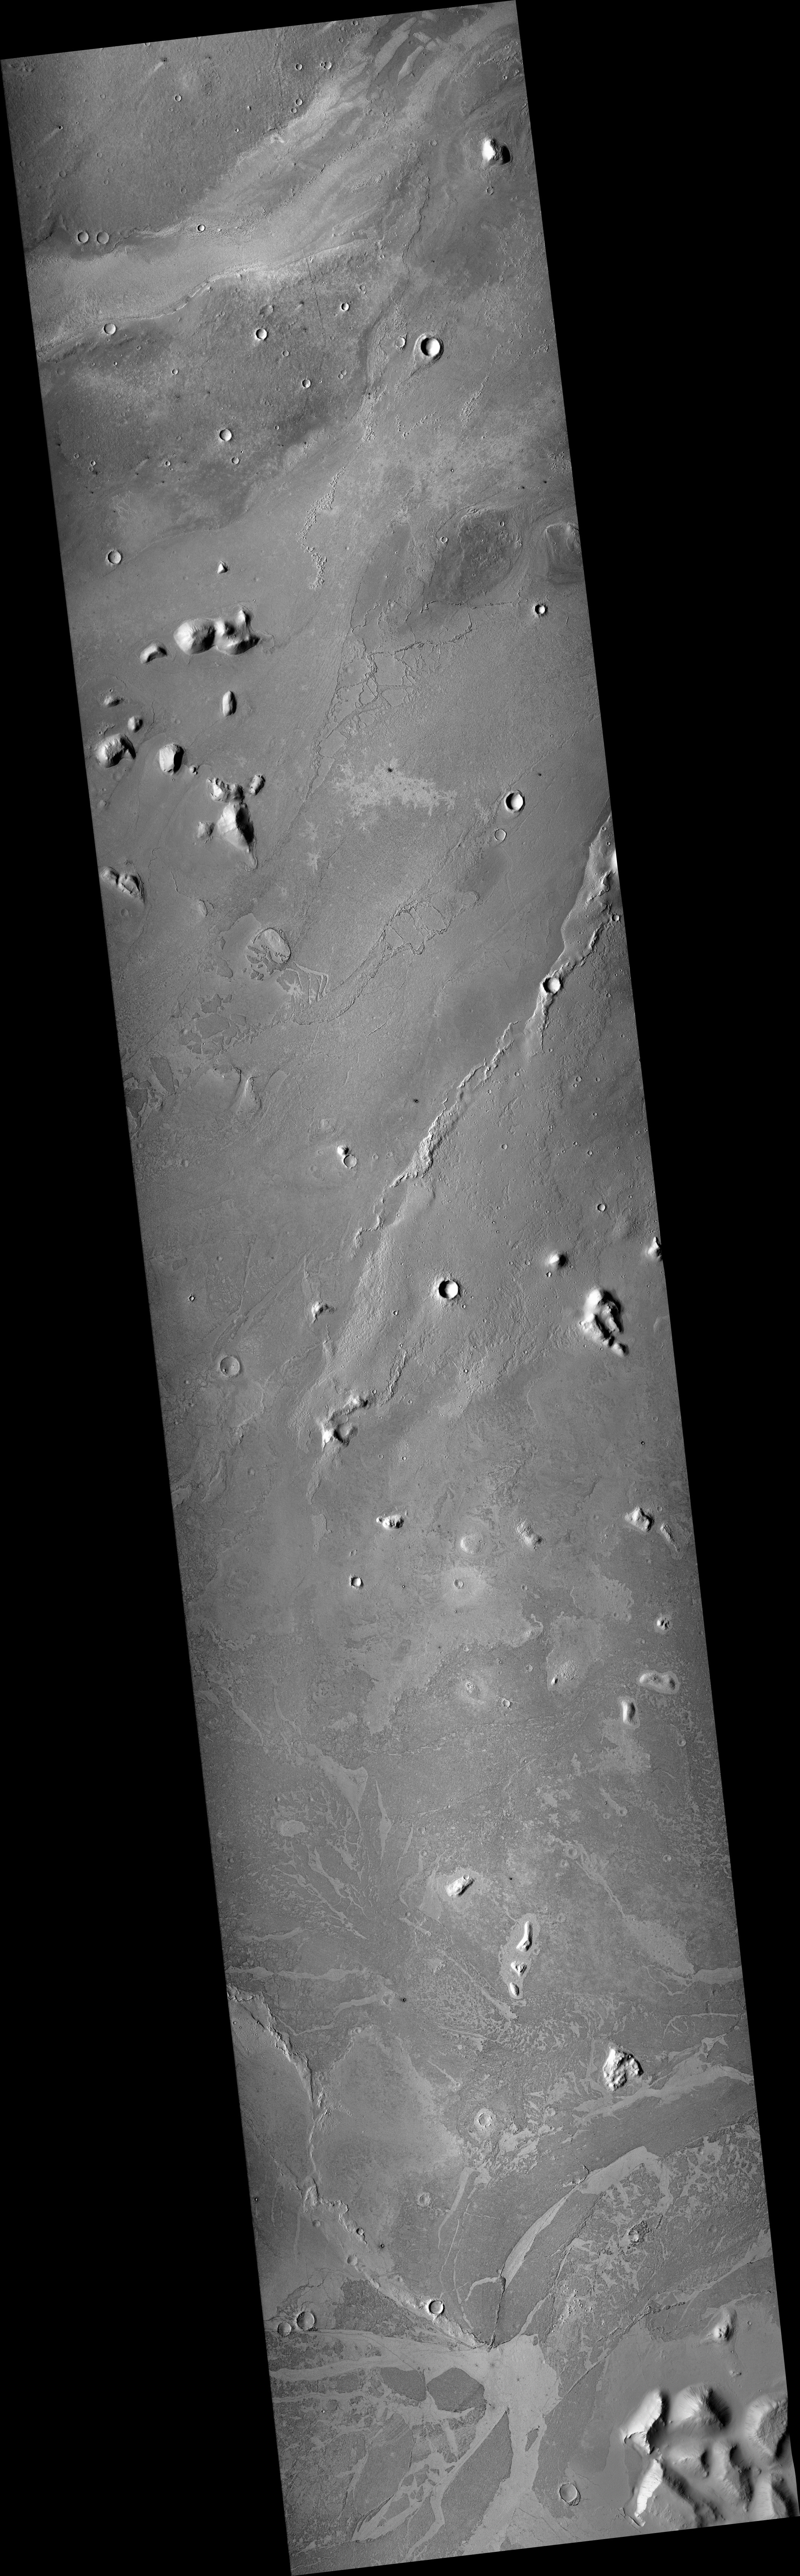
\includegraphics[height=.6\textheight, keepaspectratio]{P03-2.jpg}
			\caption{Beispiel für einen \enquote{CTX-Streifen}\footnotemark[1]}
		\end{figure}
	\end{column}
\end{columns}	
\footnotetext[1]{\bibentry{doi:10.1029/2006JE002808}}
\end{frame}

\begin{frame}{Problemstellung: Ziel}
\begin{columns}
	\begin{column}{.4\textwidth}
		Ziel ist eine möglichst genaue Segmentierung der Marsoberfläche
		\begin{itemize}
			\item Unterscheidung zwischen verschiedenen \enquote{Features} wie Krater, helle/dunkle Dünen, Berge, $\ldots$
			\item Keine manuelle Definition dieser Features
			\item Möglichst effizient, ohne menschliche Überwachung
		\end{itemize}
	\end{column}
	\begin{column}{.6\textwidth}
		\begin{figure}[H]
			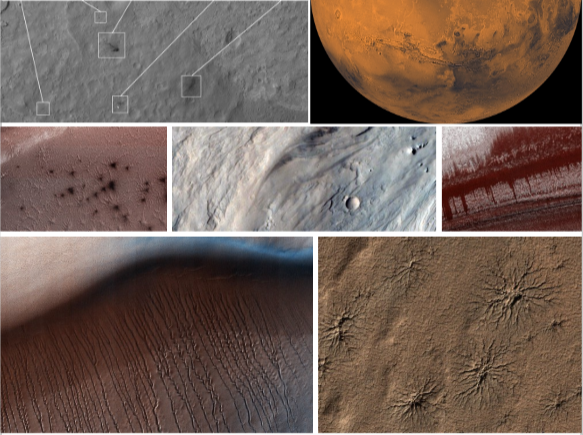
\includegraphics[width=\textwidth, keepaspectratio]{surface.png}
			\caption{Anomalien der Marsoberfläche, aus \footnotemark[1]}
		\end{figure}
	\end{column}
\end{columns}	
\footnotetext[1]{\bibentry{sheriff_2019}}
\end{frame}

\section{Vorgehensweise}

\begin{frame}{Vorgehensweise: Implementierung}
\begin{itemize}
	\item Grundlegende Idee ähnlich zu Kanezaki, basierend auf PyTorch
	\item Benutzung von Python Bibliotheken nicht immer möglich (zu große Eingabedaten, bspw. bei SLIC)
	\item[$\Rightarrow$] Speichereffizienter neu implementieren, ggf. über Sliding-Window-Verfahren
	\item Für bessere Performance wird oft auf Cython\footnotemark[1] zurück gegriffen
\end{itemize}
\footnotetext[1]{\bibentry{behnel2010cython}}	
\end{frame}

\begin{frame}{Vorgehensweise: Erweiterung}
Zur Optimierung der Ergebnisse werden einzelne Teile des Algorithmus ersetzt:
\begin{itemize}
	\item Ersetzen des relativ einfachen Neuronalen Netzes durch größere, bspw. FCNs, SegNet, DeepLabv3, etc.
	\item Ersetzen des SLIC Clusteringalgorithmus durch klassische Clusteringalgorithmen wie k-Means Clustering oder Mean-Shift Clustering
\end{itemize}
\end{frame}

\begin{frame}{Vorgehensweise: Evaluierung (1)}
Um die Alternativen evaluieren zu können, wird der Algorithmus auf Datensätze mit vorhandenen Ground Truths angewandt:
\medskip
\begin{itemize}
	\item \textit{Common Objects In Context}\footnotemark[1]
	\item \textit{Cityscapes Dataset}\footnotemark[2]
	\item[$\Rightarrow$] Weit verbreitete Datensätze zur Bildsegmentierung
	\medskip
	\item \textit{The Prague Texture Segmentation Datagenerator and Benchmark}\footnotemark[3]
	\item[$\Rightarrow$] Zufällig generierte Datensätze zur Clusteringanalyse
	\medskip
	\item \textit{Crater Dataset} der UMass Boston
	 KDLab\footnotemark[4]
	\item[$\Rightarrow$] Den zu analysierenden Daten sehr ähnlich, also realitätsnaher
\end{itemize}
\footnotetext[1]{\bibentry{LMBHPRDZ:ECCV:2014}}	
\footnotetext[2]{\bibentry{Cordts2016Cityscapes}}	
\footnotetext[3]{\bibentry{mikevs2015benchmarking}}	
\footnotetext[4]{\bibentry{umass_craters}}	
\end{frame}

\begin{frame}{Vorgehensweise: Evaluierung (2)}
	TODO
\end{frame}

\begin{frame}{Vorgehensweise: Evaluierung (3)}
Die generierten Resultate werden mit den jeweils zugehörigen Ground Truths verglichen, bspw. über den Rand Index:
\[R = \frac{a+b}{\binom{n}{2}}\]
mit
\begin{itemize}
	\item{$a=$} Anzahl Paare die in beiden Segmentierungen in gleichen Clustern liegen
	\item{$b=$} Anzahl Paaren die in beiden Segmentierungen in unterschiedlichen Clustern liegen
	\item{$n=$} Anzahl Elemente
\end{itemize}
\bigskip
Es existieren noch weitere Evaluierungsmethoden, wie z.B. Intersection over Union
\pause
\bigskip
\begin{block}{Hinweis}
	Metriken, die auf Clusterlabels basieren sind nur eingeschränkt nutzbar
\end{block}
\pause
\bigskip
\begin{block}{Hinweis}
	Zum Vergleich von NNs müssen diese jeweils den selben Seed nutzen
\end{block}
\end{frame}

\begin{frame}{Vorgehensweise: Optimierungen}
	\begin{itemize}
		\item Eingabebilder in Graustufen: Optimierung des Clusterings und des NNs
		\item Ggf. Verkleinerung der Eingabebilder wenn dies keine starke Degradierung der Analyse ergibt
		\item Parallelisierung entweder pro Bild oder mehrere Bilder parallel
		\item Wahl eines geeigneten Clustering-Algorithmus
		\item Wahl des am besten geeigneten Aufbaus des NNs
		\item Image Preprocessing, bspw. zum Zuschneiden der Streifen
	\end{itemize}
\end{frame}
\end{document}